% ==========================================================================================
% PART III : masked (absorbing-state) discrete diffusion
% ==========================================================================================
\part{A masked diffusion model}

\section{Idea: learn to un-mask}\label{sec:md_idea}
The Potts models of Part~II had to write the distribution in a fixed form, $e^{-E(\s)}/Z$, and were trained by
pseudo-likelihood, which never sees $Z$. We saw what that costs: wrong family weights. A diffusion model takes a
different route. It never writes $P(\s)$ explicitly. Instead it learns to \emph{undo a corruption}:
\begin{enumerate}[nosep]
\item \textbf{Forward (corruption)}: take a real sequence and hide more and more of its residues behind a special
      symbol \texttt{[M]} (``mask''), until everything is hidden.
\item \textbf{Reverse (generation)}: a neural network, the \emph{denoiser}, looks at a partially hidden sequence and
      says, for every hidden site, how likely each amino acid is. Starting from a fully hidden sequence and revealing
      sites one after another with these probabilities generates a new sequence.
\end{enumerate}
Because \texttt{[M]} is a state the forward process can enter but never leave, this is called
\emph{absorbing-state} (or \emph{masked}) diffusion. We follow the MDLM formulation (Sahoo et al., 2024). The network
outputs probabilities directly and no couplings are involved. The training loss is a bound on the true
log-likelihood $-\log p_\theta(\s)$, which, unlike the pseudo-likelihood, includes the global normalisation.

\section{The forward process}\label{sec:md_forward}
Extend the alphabet with one symbol, \texttt{[M]} (index $q=20$). A \emph{noise level} $t\in[0,1]$ sets how much is
hidden through a decreasing function $\alpha_t$ with $\alpha_0=1$, $\alpha_1=0$. We use the linear schedule
$\alpha_t=1-t$. Each site is corrupted \emph{independently}:
\begin{equation}\label{eq:md_forward}
q(x^i_t\mid x^i_0)=\alpha_t\,\one[x^i_t=x^i_0]+(1-\alpha_t)\,\one[x^i_t=\texttt{[M]}],\qquad
q(\bm x_t\mid\bm x_0)=\prod_{i=1}^Lq(x^i_t\mid x^i_0).
\end{equation}
At time $t$ each site is still visible with probability $\alpha_t=1-t$ and hidden with probability $t$; at $t=1$
everything is hidden. \texttt{test\_13} checks that the fraction of masked sites equals $t$ and that visible sites are untouched.

\paragraph{From $s$ to $t$ ($s<t$).} A site visible at $s$ must stay visible until $t$. Since $\alpha_t=\alpha_s\cdot(\alpha_t/\alpha_s)$,
the process is a Markov chain in which a visible site survives from $s$ to $t$ with probability $\alpha_t/\alpha_s$ and a
masked site stays masked forever:
\[
q(x^i_t\mid x^i_s)=\begin{cases}\alpha_t/\alpha_s & x^i_t=x^i_s\neq\texttt{[M]}\\ 1-\alpha_t/\alpha_s & x^i_t=\texttt{[M]},\ x^i_s\neq\texttt{[M]}\\ 1 & x^i_t=x^i_s=\texttt{[M]}.\end{cases}
\]
Equivalently, every site is hidden at an independent random time, uniformly distributed on $[0,1]$ for the
linear schedule. We use this picture for the sampler.

\section{The reverse process}\label{sec:md_reverse}
\subsection{If we knew the clean sequence: the exact posterior}
Consider one site that is hidden at time $t$. What was it at an earlier time $s<t$? By Bayes' rule,
$q(x^i_s\mid x^i_t,x^i_0)\propto q(x^i_t\mid x^i_s)\,q(x^i_s\mid x^i_0)$. Given $x^i_t=\texttt{[M]}$, there are only two
possibilities for $x^i_s$:
\begin{itemize}[nosep]
\item $x^i_s=\texttt{[M]}$: weight $1\cdot(1-\alpha_s)$;
\item $x^i_s=x^i_0$ (visible at $s$, hidden between $s$ and $t$): weight $(1-\alpha_t/\alpha_s)\cdot\alpha_s=\alpha_s-\alpha_t$.
\end{itemize}
The two weights sum to $1-\alpha_t$, so
\begin{equation}\label{eq:md_posterior}
\boxed{\;q(x^i_s\mid x^i_t=\texttt{[M]},x^i_0)=\frac{1-\alpha_s}{1-\alpha_t}\,\one[x^i_s=\texttt{[M]}]
+\frac{\alpha_s-\alpha_t}{1-\alpha_t}\,\one[x^i_s=x^i_0]\;}
\end{equation}
and a visible site simply stays: $q(x^i_s\mid x^i_t\neq\texttt{[M]})=\one[x^i_s=x^i_t]$. For the linear schedule the
probability of being revealed between $t$ and $s$ is $\frac{\alpha_s-\alpha_t}{1-\alpha_t}=\frac{t-s}{t}$.

\subsection{The model: replace the unknown $x_0$ by the denoiser}
At generation time $x^i_0$ is unknown. The model keeps the form \eqref{eq:md_posterior} and replaces the indicator
$\one[x^i_s=x^i_0]$ by the network's guess:
\begin{equation}\label{eq:md_model}
p_\theta(x^i_s\mid\bm x_t)=\frac{1-\alpha_s}{1-\alpha_t}\,\one[x^i_s=\texttt{[M]}]+\frac{\alpha_s-\alpha_t}{1-\alpha_t}\,
\underbrace{p_\theta(x^i_0=x^i_s\mid\bm x_t,t)}_{\text{denoiser}}\qquad(x^i_t=\texttt{[M]}),
\end{equation}
where the \textbf{denoiser} $p_\theta(x^i_0=a\mid\bm x_t,t)$ is a probability distribution over the 20 amino acids
for every hidden site, computed by a neural network that sees the whole partially hidden sequence. Two
constraints are built in (the ``SUBS'' parametrisation): the denoiser puts no probability on \texttt{[M]} (its
output layer has 20 entries), and visible sites are never changed.

\subsection{What should the denoiser output? The optimal denoiser}\label{sec:md_optimal}
Suppose the network could be anything. For a given $\bm x_t$, the best answer is the true conditional probability
of the clean residue given everything that is visible. By Bayes' rule and \eqref{eq:md_forward},
\[
p(\bm x_0\mid\bm x_t)\propto p(\bm x_0)\,q(\bm x_t\mid\bm x_0)
=p(\bm x_0)\,\alpha_t^{\#\text{visible}}(1-\alpha_t)^{\#\text{hidden}}\;\one[\bm x_0\text{ agrees with }\bm x_t\text{ on the visible sites}].
\]
The factor $\alpha_t^{\#\text{visible}}(1-\alpha_t)^{\#\text{hidden}}$ is the same for every $\bm x_0$ compatible with
$\bm x_t$, so it cancels in the normalisation:
\begin{equation}\label{eq:md_opt}
\boxed{\;p^\star(x^i_0=a\mid\bm x_t,t)=P\big(x^i=a\ \big|\ \text{the visible sites of }\bm x_t\big)\;}
\end{equation}
It \textbf{does not depend on $t$}: the masking is independent of the residues, so the noise level carries no
information about them. (We nevertheless give $t$ to the network, as you chose. This is the classic design, and
it lets us check empirically that the network learns to ignore it.) Two special cases connect with the rest of
this document:
\begin{itemize}[nosep]
\item everything hidden: $p^\star(x^i_0=a\mid\texttt{[M]}\dots\texttt{[M]})=f_i(a)$, the single-site frequencies;
\item only site $i$ hidden: $p^\star=P(x^i=a\mid\bm x_{-i})$, exactly the conditional that the pseudo-likelihood of
      Part~II fits. For our data it is the Potts conditional \eqref{eq:cond} of the clade the sequence came from.
\end{itemize}
So the network \textbf{directly outputs probabilities}. \texttt{test\_14} verifies both special cases on a tiny Potts model
where the exact answers are known, and \texttt{s10} measures the second one on the real test sequences.

\section{The loss: a bound on the likelihood}\label{sec:md_elbo}
\subsection{From the ELBO to a weighted cross-entropy}
Divide $[0,1]$ into $T$ steps $t_k=k/T$. The standard variational bound of a diffusion model (the evidence lower
bound, ELBO) reads
\begin{align*}
-\log p_\theta(\bm x_0)\le{}&\underbrace{\mathrm{KL}\big(q(\bm x_1|\bm x_0)\,\|\,p(\bm x_1)\big)}_{=0}
+\underbrace{(\text{reconstruction at }t=0)}_{=0}\\
&+\sum_{k=1}^{T}\E_{q(\bm x_{t_k}|\bm x_0)}\Big[\mathrm{KL}\big(q(\bm x_{t_{k-1}}|\bm x_{t_k},\bm x_0)\,\|\,p_\theta(\bm x_{t_{k-1}}|\bm x_{t_k})\big)\Big].
\end{align*}
(The derivation is the usual one: write $\log p_\theta(\bm x_0)=\log\E_q[p_\theta(\bm x_{0:1})/q(\bm x_{t_1:1}\mid\bm x_0)]$ and
apply Jensen's inequality $\log\E\ge\E\log$.) The first term vanishes because at $t=1$ everything is masked for
both $q$ and the model. The last vanishes because at $t=0$ nothing is masked. Each KL is a sum over sites (the
site-wise factorisation of \eqref{eq:md_posterior}, \eqref{eq:md_model}). For a site visible at $t$ both
distributions are the same point mass, so KL $=0$. For a hidden site, both put the \emph{same} mass
$\frac{1-\alpha_s}{1-\alpha_t}$ on \texttt{[M]}; $q$ puts the rest on $x^i_0$, and the model spreads it as
$\frac{\alpha_s-\alpha_t}{1-\alpha_t}\,p_\theta(\cdot\mid\bm x_t)$. Hence
\begin{align*}
\mathrm{KL}&=\frac{1-\alpha_s}{1-\alpha_t}\underbrace{\log\frac{(1-\alpha_s)/(1-\alpha_t)}{(1-\alpha_s)/(1-\alpha_t)}}_{=0}
+\frac{\alpha_s-\alpha_t}{1-\alpha_t}\log\frac{(\alpha_s-\alpha_t)/(1-\alpha_t)}{\big[(\alpha_s-\alpha_t)/(1-\alpha_t)\big]\,p_\theta(x^i_0\mid\bm x_t)}\\
&=\frac{\alpha_s-\alpha_t}{1-\alpha_t}\,\big(-\log p_\theta(x^i_0\mid\bm x_t)\big).
\end{align*}
Summing over the $T$ steps and letting $T\to\infty$, $\alpha_{t_{k-1}}-\alpha_{t_k}\to-\alpha'_t\,dt$ and the sum becomes an
integral:
\begin{equation}\label{eq:md_nelbo}
-\log p_\theta(\bm x_0)\le\mathcal L_{\text{NELBO}}(\bm x_0)=\int_0^1\frac{-\alpha'_t}{1-\alpha_t}\;
\E_{\bm x_t\sim q(\cdot|\bm x_0)}\Big[\sum_{i:\,x^i_t=\texttt{[M]}}-\log p_\theta(x^i_0\mid\bm x_t,t)\Big]dt ,
\end{equation}
and for the linear schedule ($-\alpha'_t=1$, $1-\alpha_t=t$):
\begin{equation}\label{eq:md_nelbo_lin}
\boxed{\;\mathcal L_{\text{NELBO}}(\bm x_0)=\E_{t\sim\mathcal U(0,1)}\,\E_{\bm x_t}\Big[\frac1t\sum_{i\text{ hidden}}-\log p_\theta(x^i_0\mid\bm x_t,t)\Big]\;}
\end{equation}
In words: \textbf{hide a random fraction $t$ of the sites, ask the network to predict the hidden residues, and
average the cross-entropy with weight $1/t$}. The weight compensates for the number of hidden sites, $\approx tL$,
so that every noise level contributes comparably. We report $\mathcal L_{\text{NELBO}}/L$ in nats per site. It is an
\emph{upper bound} on $-\log p_\theta(\bm x)/L$, the true negative log-likelihood per site. Unlike the pseudo-likelihood,
it therefore involves the full normalisation.

\subsection{Why the bound can be tight}
With the optimal denoiser \eqref{eq:md_opt}, the bound becomes an equality in expectation:
$\E\,\mathcal L_{\text{NELBO}}(\bm x)=-\log p(\bm x)$. The intuition goes through the sampler of \S\ref{sec:md_sampler}. It
reveals the sites in a uniformly random order $\sigma$ and draws each from the denoiser. With the exact conditionals,
every ordering reproduces $p(\bm x)$ through the chain rule,
$p(\bm x)=\prod_kP(x^{\sigma_k}\mid x^{\sigma_1},\dots,x^{\sigma_{k-1}})$, and the NELBO is the average over orderings of
$-\log$ of this product. \texttt{test\_13} checks numerically, on a tiny Potts model with an exact denoiser built by
enumeration, that the NELBO equals the entropy of the distribution.

\subsection{Practical details}
\begin{itemize}[nosep]
\item \textbf{Variance reduction}: within a batch of $B$ sequences the times are stratified, $t_b=(u+b/B)\bmod1$ with a
      single $u\sim\mathcal U(0,1)$, and clipped to $[10^{-3},1]$ (the $1/t$ weight is large near 0).
\item \textbf{Optimiser}: AdamW, learning rate $3\times10^{-4}$ with 1000 warm-up steps, gradient clipping at 1, batch 256,
      mixed precision (fp16 with gradient scaling, on the GPU's tensor cores).
\item \textbf{EMA}: we keep an exponential moving average of the weights, $\bar\theta\leftarrow0.999\,\bar\theta+0.001\,\theta$ after
      every step, and evaluate and save $\bar\theta$ (a standard stabiliser for diffusion models).
\item \textbf{Validation}: $\mathcal L_{\text{NELBO}}/L$ on the 18{,}000 validation sequences, with the \emph{same} random times and
      masks at every epoch (4 draws per sequence), for early stopping (patience 15, at most 150 epochs).
\end{itemize}

\section{Sampling}\label{sec:md_sampler}
\paragraph{Ancestral sampler with $T$ steps.} Start from $\bm x_1=\texttt{[M]}\cdots\texttt{[M]}$. For $t=1,1-\frac1T,\dots,\frac1T$ and
$s=t-\frac1T$: for every hidden site, reveal it with probability $\frac{t-s}{t}$ (eq.~\eqref{eq:md_posterior}), drawing
its residue from the denoiser $p_\theta(\cdot\mid\bm x_t,t)$. At the last step ($s=0$) every remaining site is revealed.
\textbf{Caveat}: sites revealed in the \emph{same} step are drawn \emph{independently} of each other, from the same $\bm x_t$. If two
correlated sites are revealed together, their correlation is lost. With $T=1$ all $L$ sites are drawn at once from
$p_\theta(\cdot\mid\text{all hidden})=f_i$: independent sites. The error disappears only when steps are so small that
sites are revealed one at a time. \texttt{test\_13} (figure below) shows this with the exact denoiser: the total-variation
error goes from the independent-sites value at $T=1$ to the sampling noise at $T\gtrsim30$ for $L=4$.

\paragraph{Exact continuous-time sampler.} The $T\to\infty$ limit can be simulated exactly. In the forward process
each site is hidden at an independent uniform time, so in reverse the sites are revealed one at a time, in a
uniformly random order, the $k$-th reveal occurring at the $k$-th largest of $L$ uniform times $\tau_{(1)}>\dots>\tau_{(L)}$.
The sampler draws those times, then for $k=1,\dots,L$ reveals the $k$-th site from $p_\theta(\cdot\mid\bm x_{\tau_{(k)}},\tau_{(k)})$.
That is \textbf{exactly $L=60$ network calls per sequence}, with no step-size error
(\texttt{continuous\_time\_sample}; \texttt{test\_13} checks that it reproduces the exact distribution). It is our main sampler.
The finite-$T$ sampler is kept to measure the step-size effect on real data ($T=15,60,240$).

\begin{figure}[H]
\centering
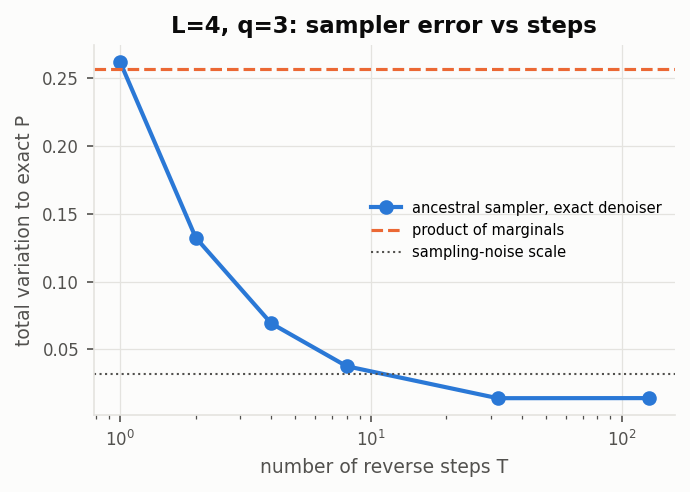
\includegraphics[width=0.48\linewidth]{tests/test_13_masked_diffusion/test_ancestral_sampler_with_exact_denoiser/tv_vs_steps.png}
\caption{\texttt{test\_13}: $L=4$, $q=3$ Potts model, exact denoiser. Distance of the ancestral sampler's output to the exact
distribution vs the number of steps $T$. $T=1$ gives the product of the marginals (independent sites); large $T$ is exact.}
\end{figure}

\section{The network}\label{sec:md_network}
The denoiser is a bidirectional transformer. Unlike the factored attention of Part~II, its attention weights
\emph{depend on the residues}, so it is not restricted to pairwise (Potts) interactions.
\begin{center}\footnotesize
\begin{tabular}{p{0.12\linewidth}p{0.5\linewidth}p{0.28\linewidth}}
\toprule
stage & operation & shape / parameters\\
\midrule
input & $\bm x_t\in\{0,\dots,19,\texttt{[M]}\}^{60}$, noise level $t\in[0,1]$ & $(B,60)$, $(B,)$\\
embedding & token emb.\ ($21\times256$) $+$ position emb.\ ($60\times256$) $+$ time emb. & $(B,60,256)$; 90{,}880 params\\
time emb. & $[\sin2\pi2^kt,\cos2\pi2^kt]_{k=0..7}\to$ Linear--GELU--Linear & (included above)\\
encoder & $6\times$[LayerNorm $\to$ self-attention (8 heads) $\to$ LayerNorm $\to$ MLP $256{\to}1024{\to}256$], with residual connections & 4{,}738{,}560 params\\
head & LayerNorm $\to$ Linear $256\to20$ & 5{,}652 params\\
output & logits of $p_\theta(x^i_0=a\mid\bm x_t,t)$ for every site & $(B,60,20)$\\
\midrule
total & & \textbf{4{,}835{,}092} parameters\\
\bottomrule
\end{tabular}
\end{center}
Each layer adds its input back (residual connections), so information can flow straight through. The LayerNorms
rescale the vectors to keep the training stable. Self-attention lets every site gather information from every
other site, with weights that depend on what is there.

\paragraph{Training data and cost.} The same 144{,}000 training sequences of all 18 clades, \textbf{without any label}
(unconditioned, as you chose), and the same validation and test splits as in Part~II. Measured on the RTX~2060:
74\,ms per step in mixed precision (181\,ms in fp32), i.e.\ $\approx45$\,s per epoch plus validation, so at most
$\approx2$\,h for 150 epochs.

\section{Tests of Part III}\label{sec:md_tests}
\begin{center}\small
\begin{tabular}{p{0.3\linewidth}p{0.62\linewidth}}
\toprule
test & what it verifies\\
\midrule
\texttt{test\_13\_masked\_diffusion} & masked fraction $=t$, visible sites untouched; stratified times; output shape (20 classes, no mass on
\texttt{[M]}); the output depends on $t$; save/load; \textbf{with the exact denoiser the NELBO equals the entropy}, and a uniform
denoiser gives $L\log q$; ancestral sampler: $T=1$ gives independent sites, large $T$ is exact; continuous-time sampler is
exact; one-site-masked readout $=$ the Potts conditional\\
\texttt{test\_14\_diffusion\_training} & a small denoiser trained on 20{,}000 samples of an $L=4$, $q=3$ Potts model (81 states):
validation NELBO within 0.03 nats/site of the exact $-\log p$ of the validation sequences; fully-masked output $=$ marginals;
one-site-masked output $=$ Potts conditionals (probability-weighted error $<0.03$); samples: total variation $0.028$ to the
exact distribution\\
\texttt{test\_15\_diffusion\_pipeline} & the whole chain (dataset $\to$ \texttt{s09} train $\to$ \texttt{s10} evaluate) on a tiny tree, with mixed precision\\
\texttt{test\_16\_checkpointing} & checkpoint files are written (best model, full state, snapshots every $N$ epochs); 4 epochs $+$ resume to 6 gives exactly the same losses and weights as 6 epochs in one go\\
\texttt{test\_10} (added case) & the pseudo-likelihood clade classifier of \texttt{s11} assigns samples of two Potts models to the right one; its score equals the sum of the log conditionals\\
\bottomrule
\end{tabular}
\end{center}

\begin{figure}[H]
\centering
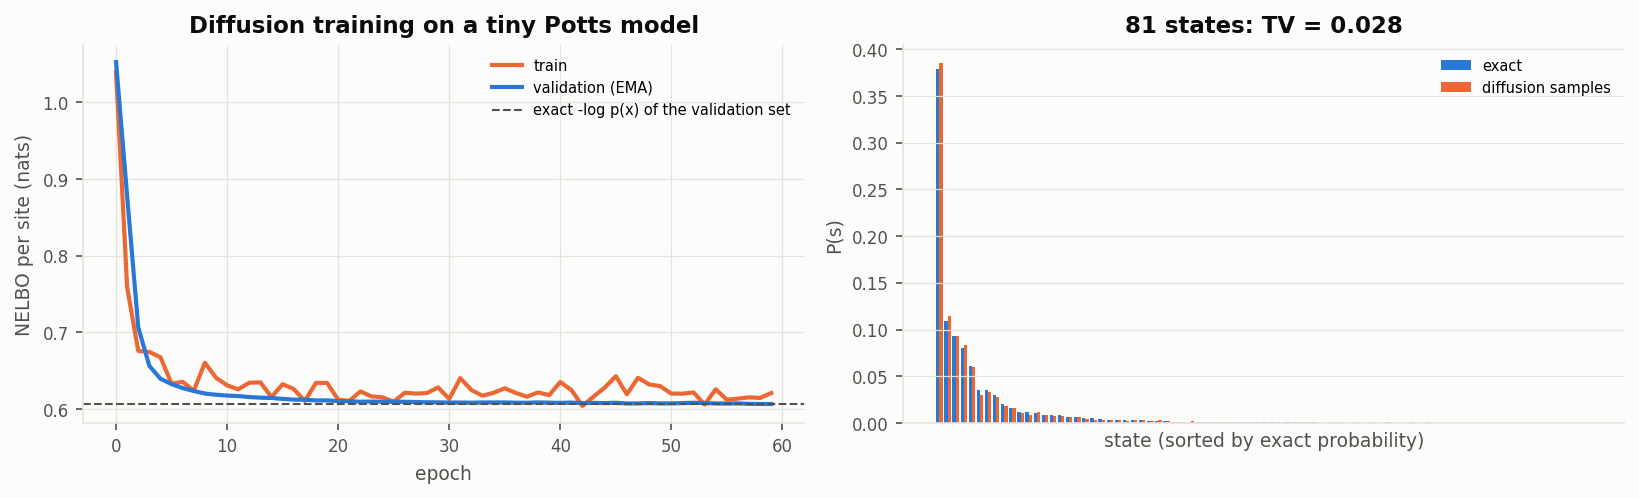
\includegraphics[width=\linewidth]{tests/test_14_diffusion_training/test_learns_tiny_potts/tiny_potts_diffusion.png}
\caption{\texttt{test\_14}. Left: training curve on the tiny Potts model; the dashed line is the exact $-\log p(\bm x)$ per site of the
validation sequences, which the bound approaches from above. Right: the 81 states, exact probability vs frequency in
20{,}000 diffusion samples.}
\end{figure}

\section{What we will measure}\label{sec:md_plan}
With the same held-out test set and the same metrics as the Potts models (\texttt{s10}):
\begin{enumerate}[nosep]
\item test NELBO per site (the likelihood bound);
\item \textbf{the probabilities themselves}: $p_\theta(x^i\mid\bm x_{-i})$ on test sequences vs the exact conditional of the true clade
      model, and the resulting pseudo-NLL per site, directly comparable with Part~II (true models 0.80, conditioned Potts
      0.873, unconditioned Potts 0.949);
\item samples: $r_f$, $r_C$, identity, \textbf{family proportions} (the main failure of the unconditioned Potts model; a likelihood
      bound should get them right), distances (novelty, diversity, Fréchet), for the continuous-time sampler and for $T=15,60,240$.
\end{enumerate}
